% This is the Reed College LaTeX thesis template. Most of the work
% for the document class was done by Sam Noble (SN), as well as this
% template. Later comments etc. by Ben Salzberg (BTS). Additional
% restructuring and APA support by Jess Youngberg (JY).
% Your comments and suggestions are more than welcome; please email
% them to cus@reed.edu
%
% See http://web.reed.edu/cis/help/latex.html for help. There are a
% great bunch of help pages there, with notes on
% getting started, bibtex, etc. Go there and read it if you're not
% already familiar with LaTeX.
%
% Any line that starts with a percent symbol is a comment.
% They won't show up in the document, and are useful for notes
% to yourself and explaining commands.
% Commenting also removes a line from the document;
% very handy for troubleshooting problems. -BTS

% As far as I know, this follows the requirements laid out in
% the 2002-2003 Senior Handbook. Ask a librarian to check the
% document before binding. -SN

%%
%% Preamble
%%
% \documentclass{<something>} must begin each LaTeX document
\documentclass[12pt,twoside]{reedthesis}
% Packages are extensions to the basic LaTeX functions. Whatever you
% want to typeset, there is probably a package out there for it.
% Chemistry (chemtex), screenplays, you name it.
% Check out CTAN to see: http://www.ctan.org/
%%
\usepackage{graphicx,latexsym}
\usepackage{amssymb,amsthm,amsmath}
\usepackage{longtable,booktabs,setspace}
\usepackage{chemarr} %% Useful for one reaction arrow, useless if you're not a chem major
\usepackage[hyphens]{url}
\usepackage{rotating}
\usepackage{natbib}
\usepackage{todonotes}
\usepackage{hyperref}
\usepackage{verbatim}
\usepackage{epigraph}
\usepackage{lmodern}
\usepackage{caption}
\usepackage{listings}
\lstset{
basicstyle=\small\ttfamily,
columns=flexible,
breaklines=true
}

%% Added for comments
\usepackage{color}
\newcommand{\anna}[1]{{\color{blue}[AR: #1]}}
\newcommand{\new}[2]{{\color{purple}#1 [#2]}}
\theoremstyle{definition}
\newtheorem{definition}{Definition}[section]

%% Preface quote stuff
\newlength\longest

%% Graphics path
\graphicspath{ {figures/} }

% Comment out the natbib line above and uncomment the following two lines to use the new
% biblatex-chicago style, for Chicago A. Also make some changes at the end where the
% bibliography is included.
%\usepackage{biblatex-chicago}
%\bibliography{thesis}

\newcommand{\argmax}{\arg\!\max}

% \usepackage{times} % other fonts are available like times, bookman, charter, palatino

\title{Prize-Collecting Steiner Trees in Directeded Signaling Hypergraphs}
\author{Barney Isaksen Potter}
% The month and year that you submit your FINAL draft TO THE LIBRARY (May or December)
\date{May 2016}


%\division{Mathematics and Natural Sciences}
\advisor{Dr. Anna Ritz}
%If you have two advisors for some reason, you can use the following
\altadvisor{Dr. James Fix}
%%% Remember to use the correct department!
\department{Interdisciplinary Committee for Mathematics \& Biology}
% if you're writing a thesis in an interdisciplinary major,
% uncomment the line below and change the text as appropriate.
% check the Senior Handbook if unsure.
\thedivisionof{The Division of Mathematics \& Natural Sciences}
% if you want the approval page to say "Approved for the Committee",
% uncomment the next line
\approvedforthe{Committee}

\setlength{\parskip}{0pt}
%%
%% End Preamble
%%
%% The fun begins:
\begin{document}

  \maketitle
  \frontmatter % this stuff will be roman-numbered
  \pagestyle{empty} % this removes page numbers from the frontmatter

% Acknowledgements (Acceptable American spelling) are optional
% So are Acknowledgments (proper English spelling)
    \chapter*{Acknowledgments}
	I want to thank a few people:

  \begin{itemize}
    \item{Mom and Dad}
    \item{Mari}
    \item{Far Far}
    \item{Sam, Will, Rich, and ext. family}
    \item{Helen and Melvin}
    \item{Michael and Caleb}
    \item{Anna and Jim}
    \item{Sarah, Jeremy, Leigh, and the Schaack Lab}
    \item{My benefactor}
    \item{A.T \& A.L} %Turing and Lovelace
  \end{itemize}

% The preface is optional
% To remove it, comment it out or delete it.
    \chapter*{Preface}
	%\epigraph{We can only see a short distance ahead, but we can see plenty there that needs to be done.}{\textit{Alan Turing}}
  \null\vfill

\settowidth\longest{\huge\itshape but we can see plenty there }
\begin{center}
\parbox{\longest}{%
  \raggedright{\huge\itshape%
   We can only see \\
  a short distance ahead, \\
  but we can see plenty there \\
  that needs to be done.\par\bigskip
  }
  \raggedleft\Large\MakeUppercase{Alan Turing}\par%
}
\end{center}

\vfill\vfill


    \tableofcontents
% if you want a list of tables, optional
    \listoftables
% if you want a list of figures, also optional
    \listoffigures

% The abstract is not required if you're writing a creative thesis (but aren't they all?)
% If your abstract is longer than a page, there may be a formatting issue.
    \chapter*{Abstract}
	The preface pretty much says it all.

	\chapter*{Dedication}
	You can have a dedication here if you wish.

  \mainmatter % here the regular arabic numbering starts
  \pagestyle{fancyplain} % turns page numbering back on

%The \introduction command is provided as a convenience.
%if you want special chapter formatting, you'll probably want to avoid using it altogether

    \chapter*{Introduction}
         \addcontentsline{toc}{chapter}{Introduction}
	\chaptermark{Introduction}
	\markboth{Introduction}{Introduction}
	% The three lines above are to make sure that the headers are right, that the intro gets included in the table of contents, and that it doesn't get numbered 1 so that chapter one is 1.

% Double spacing: if you want to double space, or one and a half
% space, uncomment one of the following lines. You can go back to
% single spacing with the \singlespacing command.
\onehalfspacing
% \doublespacing

Since the discovery of cells by Robert Hooke in 1665, biologists have worked tirelessly to unlock the mysteries of cell function. Over the last half-century, our knowledge of how cells function has grown tremendously. An important and growing part of this field has been the growing use of computational methods in helping researchers to both test pre-existing hypotheses, and generate novel hypotheses. Computer-based methods have a wide range of applications, from DNA and RNA sequence analysis (\cite{humanGenome}) to high-throughput modeling of population growth (\cite{SomethingRelevant}), to the growing fields concerned with artificial neural networks (\cite{SomethingElse}). Importantly, in recent years, biologists\footnote{And other scientists, for that matter.} have begun to employ some of the computational tools that computer scientists have been developing for decades. This recent synthesis of fields (see Figure \ref{fig:bioinf_venn}) has created a new area of research, where existing algorithms and computational methodologies are being adapted and tweaked to help elucidate new meaning from biological data.\par

 \begin{figure}[h]
   \begin{center}
     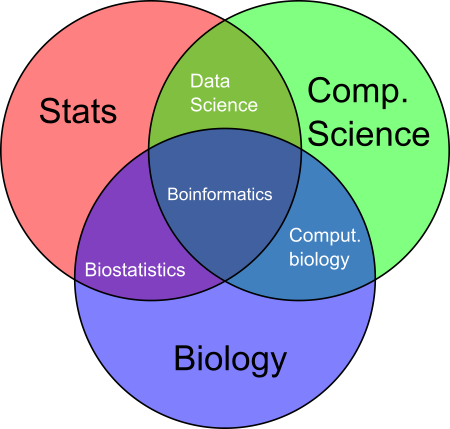
\includegraphics[width=\textwidth/2]{bioinformatics_venn}
   \caption[Bioinformatic fields.]{A venn diagram of the intersection between the fields of biology, computer science, and statistics {\cite{putIntoBib}}. This thesis is primarily concerned with the field of computational biology.}
   \label{fig:bioinf_venn}
   \end{center}
 \end{figure}

 \section{Signaling Pathways}

 One of the most interesting areas where computational methods are now being applied is in the study of signaling pathways within cells. Generally, signaling pathways are representations of what we currently know about how proteins and small molecules interact within cells in order to propagate signals throughout the cell, and ultimately change the cell's behavior. We find cell signaling pathways interesting because understanding how signaling information spreads throughout a cell helps us to better understand what disregulations can result in changes in cell dynamics, which often manifest themselves in heterogenous diseases such as cancer\footnote{As well as many other diseases in which signaling pathway disregulations have been implicated.} (\cite{cancer}). Signaling pathways have been studied for years, and they have often been represented visually as flow diagrams (add a picture), but recently, researchers have begun to ``convert" the traditionally drawn digrams of signaling pathways into mathematically intersting structures, for which known algorithms can be employed to learn more about the signaling pathways.

 \section{Network Representations}

  To build a mathematical model of cell signaling pathways, we often use a graph as a data structure that is representative of the structure of the pathways. Graphs are a data structure first described by Euler in 1736 (\cite{Shields2012}) to help explain the complex relationships between objects\footnote{In Euler's case, the seven bridges of K\"{o}nigsberg.} in a concise, well defined way. For the purpose of this thesis, the word ``graph\footnote{A term coined by James Joseph Sylvester in 1878 (\cite{Biggs1986}).}" will refer to the data structure. A graph, $G=(V,E)$ is a structure that represents a set of objects, $V$ referred to as \textit{nodes} or \textit{vertices} and pairwise connections between them, $E$ referred to as \textit{edges}. Edges in a graph can either be \textit{undirected} or \textit{directed} (shown in Figure \ref{fig:simple_graph_du}), meaning that they go from one node (the \textit{tail}) to another node (the \textit{head}). We define a \textit{subgraph}, $G^\prime$, of $G$ as $G^\prime=((V^\prime,E^\prime | V^\prime \subseteq V \text{ and } E^\prime \subseteq E))$. Furthermore, we define an \textit{induced subgraph} as the subgraph that arises from a subset of edges, $E^{\prime\prime}$, and their respective heads and tails.\par

  One of the greatest advantages of using graphs as modeling tools is the wealth of graph algorithms that have been invented since Euler first proposed problems on graphs in 1736. These algorithms make it simple for graphs that are representative of real biological data to be queried for informative (i.e. shortest path between two nodes, modularity of a graph, or subgraphs that satisfy certain parameters) which can themselves be analyzed to determine whether they represent a biologically meaningful phenomena.\par

  \begin{figure}[!h]
    \begin{center}
      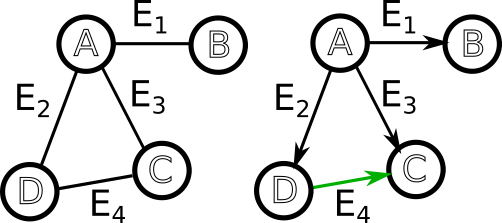
\includegraphics[width=\textwidth/2]{simple_graph_du}
    \caption[Undirected \& Directed Graphs]{A simple undirected graph (left) and it's directed counterpart (right). The green edge has node $D$ as its tail and $C$ as its head.}
    \label{fig:simple_graph_du}
    \end{center}
  \end{figure}

   \subsection{Walks, Paths, Connectivity, and Trees}

   In graphs, it is useful to define a way to traverse the graph, through the nodes and edges. We define a \textit{walk} in a graph as an alternating series of nodes and edges, such that each edge included in the walk is adjacent to the two nodes incident upon it. An example of one such walk, $\mathcal{W}$ in the undirected graph from Figure \ref{fig:simple_graph_du} is:\par

   \begin{equation*}
     \mathcal{W} = (A,E_2,D,E_2,A,E_1,B)
   \end{equation*}

   Furthermore, we can define a \textit{directed walk} in a directed graph as a walk that respects the direction of the edges in the graph. Additionally, we define a \textit{path} (or a \textit{directed path}, in directed graphs) as a walk for which there are no repeated vertices or edges. If we want to talk about a path $\mathcal{P}$ that goes from one node, $s$ to another $t$, we use the notation $\mathcal{P}(s,t)$ to describe the start and endpoints of the path. Furthermore, we say that a graph is \textit{connected} if, for any pair of nodes in the graph, there exists a path between those two nodes. It is important to note that the endpoints of both paths and walks are always nodes, not edges. For example, in the directed graph shown in Figure \ref{fig:simple_graph_du}, one possible path from $A$ to $C$, is:\par

   \begin{equation*}
     \mathcal{P}(A,C) = (A,E_2,D,E_4,C)
   \end{equation*}

   Using our definition of a path, we can also define a \textit{cycle} as a path for which the start and end nodes are the same. Using this definition, we can also say that any path or graph that does not contain any cycles as an \textit{acyclic} path or graph. Finally, we can define a \textit{tree} as any graph that is connected and acyclic. This means that for any pair of nodes in a tree there exists exactly one path between them.\par

   \subsection{Spanning Trees and Steiner Trees}

   It is often useful to construct subgraphs from a given graph that fulfill specific parameters. These subgraphs are often formulated as a decision question: ``Given a graph $G$ and a set of parameters, does subgraph $G^\prime$ of $G$ exists that meets all of the specified parameters." An example of one such graph is a complete graph, shown in Figure \ref{fig:complete_graphs}. A complete graph of $n$ nodes (\textit{k}-$n$) is defined as an undirected graph for which each node is connected to each other node by exactly one edge.

   \begin{figure}[!h]
     \begin{center}
       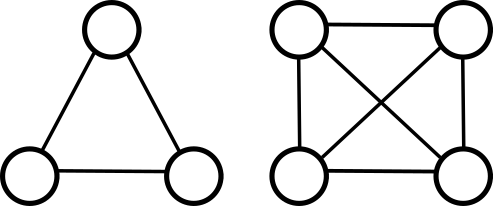
\includegraphics[width=\textwidth/2]{complete_graphs}
     \caption[Complete Graphs \textit{k}-3 and \textit{k}-4.]{The complete graphs with three and four nodes.}
     \label{fig:complete_graphs}
     \end{center}
   \end{figure}

   \paragraph{Spanning Trees.}One useful structure that we can look for in a graph is a \textit{spanning tree}. Given a graph $G=(V,E)$, we say that there exists a spannning tree if there exits some tree $\mathcal{T}=(V^\prime,E^\prime)$ for which $V^\prime = V$.  More plainly, given a graph, a spanning tree is one that ``hits" every node in the graph while still conforming to all the constraints that define a tree.

   \paragraph{Steiner Trees.}While spanning trees are useful substructures, sometimes we want to find a subtree that only spans a subset of the nodes in a graph.

 \section{Optimization}

  \subsection{Prize Collecting Steiner Trees}

 \section{Integer Linear Programming}

  For this thesis, we use a type of programming known as \textit{integer linear programming}. Integer linear programs (ILPs) solve for the optimal solution(s) to an objective expression, subject to a set of linear constraints (\cite{Papadimitriou1998}). In our case, the set of variables, $\mathbf{x}$, are all binary variables, which will represent whether a given part of the graph is included in the solution. If variable $\mathbf{x}_i$ is equal to 0 in the solution, the part of the graph with which it is associated will not be present in the optimal solution. Similarly, if $\mathbf{x}_i$ is equal to 1, its associated graph component is present in the optimal solution.\par

  The canonical form of an ILP is:\par

  \begin{align}
    \text{Maximize: }\quad&\mathbf{c^Tx}\label{eq:obj_canonical}\\
    \text{Subject to: }\quad&\mathbf{Ax}\leq\mathbf{b}\text{,}\label{eq:constA}\\
    &\mathbf{x} \geq 0 \text{,}\label{eq:constB}\\
    \text{and } \quad & \mathbf{x} \in \mathbb{Z}^n \label{eq:constC}
  \end{align}

  In this form $\mathbf{x}$ is the vector of binary variables for which the program is solving, $\mathbf{c}$ and $\mathbf{b}$ are vectors and $\mathbf{A}$ is a matrix, all of which have integers as values. For this thesis IBM ILOG CPLEX Optimization Studio (CPLEX) was used to optimize input ILPs which were input in the form of LP files (\texttt{.lp}, see Appendix B).

 \section{Goals of this Thesis}

 The goal of this thesis is to generate an algorithm that will create subnetworks in a generalization of a graph called a \textit{hypergraph}\footnote{This will be defined both informally and formally later.}. The sub-hypergraph generated by this algorithm should use weights on the edges and nodes of the hypergraph to find a subnetwork that will minimize the total cost of edges while maximizing the value of nodes. Furthermore, the output should not contain disconnected subgraphs, and it should have some sort of ``flow" going from an undetermined (i.e. not pre-specified) set of hypernodes, $S$ to another set of hypernodes, $T$. In addition to formally defining and solving for this target subnetwork, this thesis will find a way to build a network from publically available signaling pathway data, and weight that network in a meaningful way using publically available data.\par

 Ultimately, this should create a software package that anyone could use to build hypergraphs from available data, and to query that hypergraph for potential hypotheses about signaling pathway disregulations, based on a weighting scheme that the user can apply easily.\par

\chapter{Cell Signaling Networks}

Cell function is governed by countless interactions between proteins, nucleic acids, lipids, carbohydrates, and many other small molecules.  The interactions between all of these components form what we call \textit{protein-protein interaction} (PPI) networks, which are responsible for almost every process within a cell (\cite{thing}). Furthermore, we often think about specific sub-networks that explain important biological phenomena (hormone secretion, transcriptional regulation of a gene, or response to a particular stimuli are all examples). We refer to these subsets of the larger PPI network as \textit{cell signaling pathways}. We use cell signaling pathways to describe how many of the most basic reactions within cells cause propagations of information, and the results of thse signals.  Some of the most important types of interactions that we see in cell signaling networks include the assembly and destruction of protein complexes, how small molecules such as ATP interact with proteins, the cascade of events that can occur after a membrane-bound protein is bound by a ligand, or where negative feedback loops exist that can have an effect on cell function.  Historically, PPI networks have been a useful tool for compiling knowledge about individual interactions that have been studied \textit{in situ}, so that larger scale patterns of interaction can be examined, and both communicated easily and analyzed algorithmically. In recent years, there has been a push to find ways to accurately model these networks so that they can be used to predict potential areas of future research (\cite{papers}), in particular, by using graph-based methods (\cite{Aittokallio2006}).\par

There are a multitude of different forms of cell signaling pathways\footnote{As well as extracellular signaling networks and metabolic cell functions that are not triggered externally.}, responsible for many types of cell functions, but we will use the example of a cell changing its gene expression in response to an external stimuli as a general model for signaling pathways. In these cases, there are a few key steps that result in signal transduction throughout the cell. First, a trans-membrane protein will undergo a conformational change in response to a particular ligand\footnote{A small molecule that typically will bind to a trans-membrant, initiating a cascade of events (i.e. the signal that starts the process).}. Typically, this signal will be some sort of messenger molecule to which the cell needs to respond. The change in conformation results in a cascade of interactions between proteins and other small molecules within the cell. Some of the changes that can result from this cascade of signaling are protein complex assembly, complex degradation, conformational changes to other proteins, phosphorylation, or dephosphorylation (among many other reactions). The ultimate result of this signaling cascade is a change in one or more transcription factors, proteins that bind to DNA, and regulate the rate of transcription of DNA to mRNA. The ultimate result of this pathway will be a change in the expression of one or more genes within the cell, and possibly the start of new signaling pathways.\par

\paragraph{Computational Methods.}
Signaling pathways are of particular importance because they are often disregulated in heterogenous diseases such as cancer (\cite{papers}). Because of this, researchers' ability to obtain accurate information about signaling pathways, and their ability to interpret that information may help them to deduce interactions whose disregulation may be implicated in a particular disease. As these networks grow and become more accurate, we will become increasingly able to develop computational methods to mine these networks for novel areas to research, that may help explain or treat heterogenous diseases. Additionally, as the databases become more complete, cross-pathway interactions may begin to be documented that would not otherwise be apparent upon studying individual pathways. The development of new computational techniques to elucidate regulatory changes in areas where different pathways, once modeled as discrete, crosstalk. If areas like these, could be identified, they could lead to new hypotheses that researchers could investigate \textit{in situ}. Furthermore, while past research has found many individual proteins and pathways that are implicated in particular diseases, our ability to observe or quantify certain elements that could be playing an important role in pathway disregulation is limited by our current sampling methods (RNA-Seq, microarray, etc). The development of more nuanced algorithms could increase our ability to implicate proteins that we cannot currently observe being disregulated because of thow protein expression in cels is currenly quantified.\par

Beyond individual signal transduction pathways, it is useful to think of the set of all known interactions, together. We refer to this object as an \textit{interactome}, and our ability to analyze it computationally could lead to discovery (or at least postulation) of completely novel signaling networks. By examining the interactome for a species, and weighting it appropriately, it may be the case that we are able to elucidate sets of interactions that had been observed separately, but actually to be correlated with each other. A simple case of this would be if we find that one signaling pathway was to lead directly into another, that is, the outputs of the first pathway were the inputs to the other. Though interactions between multiple networks as simple as that are likely to have already been observed, it could be the case that an algorithm could find that there is some ``chain" of connections between one network and another, or that there was some form of crosstalk between some of the components of two networks. If we could find this type of interaction, it would help researchers understand the extent to which a change in one network may affect another.\par

\begin{figure}[h]
  \begin{center}
    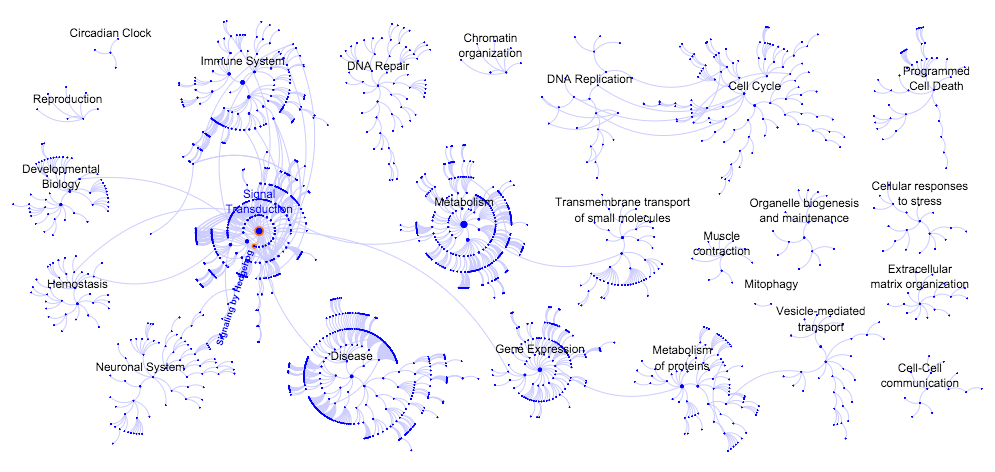
\includegraphics[width=\textwidth]{human_interactome}
  \caption[Human interactome]{The entire human interactome, as displayed by the Reacome interactive pathway browser.}
  \label{fig:human_interactome}
  \end{center}
\end{figure}

\section{PPI Databases}

In recent years, there has been a push to start curating what is already known about cell signaling, and publishing these networks online (\cite{Bauer-Mehren2009}, \cite{Cusick2009}). Many of these databases have been made available to the public, so that the data that they contain can be used collaboratively by anyone. Some of these networks are the Reactome database (\texttt{reactome.org}; \cite{Matthews2009}), NetPath (\texttt{netpath.org}; \cite{Kandasamy2010}), and SPIKE (\path{http://spike.cs.tau.ac.il/spike2/}; \cite{Paz2011}).\par
The purpose of signaling pathway databases is twofold: to create repositories of known interactions, so that they can be easily referred to and viewed in a zoomable, searchable manner (\cite{Hu2007}), and so that researchers can take advantage of the computational tools that alerady exist to find novel areas of research from these manually-curated networks (\cite{Karlebach2008}, \cite{Battle2010}). These more modern pathway interaction databases are much smaller than their earlier, non-curated counterpart, but contain much higher confidence interactions, making them better candidates for applying computational methods.\par

\section{Signaling by \emph{Hedgehog}: A Case Study}

One example of a cell signaling pathway that has a variety of biological consequences is the \textit{Hedgehog} (Hh) signal transduction network. Hedgehog is a protein that helps regulate limb formation during early development, cell development, differentiation, and the development of neural tubes (\cite{Hui2011}). Hedgehog has been implicated in the development of basal cell carcinoma\footnote{Basal cell carcinoma is thought to be the most common form of cancer in humans\cite{paper}. Indeed the author of this thesis was diagnosed with and treated for BCC.} (BCC) when it is overexpressed (\cite{Beachy2004}). Additionally, it has been shown that Hh has powerful effects on the proper layout and development of tissues in mammals, and it has been proposed that Hh is responsible for assisting with stem cell assisted tissue regeneration in adult mammals (\cite{thing}).

\begin{figure}[h]
  \begin{center}
    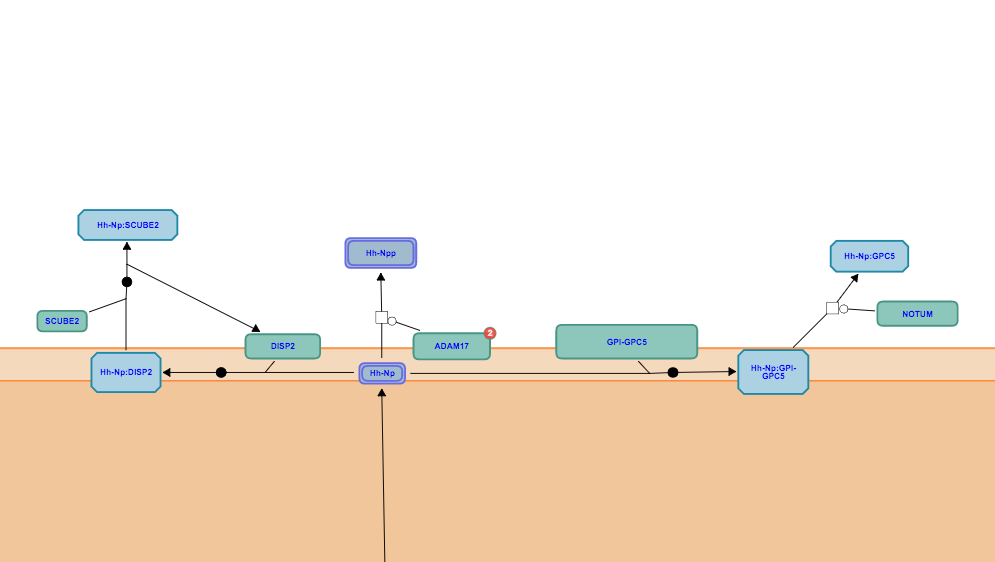
\includegraphics[width=\textwidth]{Hh-Np_secretion}
  \caption[Hedgehog secretion in \textit{Homo sapiens}]{Hh-Np secretion, as shown by \texttt{reactome.org} in \textit{Homo sapiens}.}
  \label{fig:Hh-Np_secretion}
  \end{center}
\end{figure}

The Hedgehog signaling pathway makes a useful example for applying computational methods and graph-based modeling, since the network is small enough to look at manually, but also complex enough that its analysis is nontrivial. Furthermore, because it has been implicated with BCC, along with many other forms of cancer, data for weighting signaling networks are available through public databases such as The Cancer Genome Atlas (\texttt{http://cancergenome.nih.gov/}). These factors make it an excellent choice as an example network for testing new hypergraph algorithms.\par

\section{Signaling Networks in \emph{Arabidopsis thaliana}}

One of the greatest strengths of computational methods is that they are generally agnostic to where their inputs come from, making them good tools for studying more than just human systems. In addition to humans, there is a wealth of data available for other species that can also be studied using PPI database mining. One such species is \textit{Arabidopsis thaliana} (mouse-ear cress), a plant in the mustard family that is commonly used as a model for plant genetics. Researchers often use \textit{A. thaliana} to examine the effects of genetic manipulation on plants, since \textit{A. thaliana} has one of the best known genomes of any plant\footnote{It is like the \textit{Drosophila melanogaster} of the plant world.}. Because of this, there is a huge quantity of data available that make implementing the same kind of algorithms that are possible in human signaling pathways in \textit{A. thaliana}.

\begin{figure}[h]
  \begin{center}
    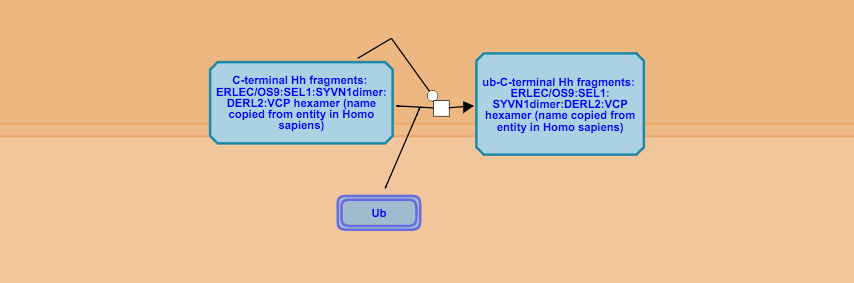
\includegraphics[width=\textwidth]{at_hh}
  \caption[\textit{Arabidopsis thaliana} Hedgehog pathway]{The Reactome Hedgehog signaling pathway in \textit{A. thaliana}. For this pathway, and many others, the Reacome database is very sparse relative to the orthologous pathways in humans, and is therefore not very useful for implementing network algorithms, at this point.}
  \label{fig:at_hh}
  \end{center}
\end{figure}

Unfortunately, for many small-scale pathways (such as the Hedgehog pathway), there is not as much pathway data available in pathway databases, since much more research has been done on humans than on any other organism. Fortunately, however, there is enough pathway data available that the overall interactome can be searched and may yield useful outcomes.\par

\begin{figure}[h]
  \begin{center}
    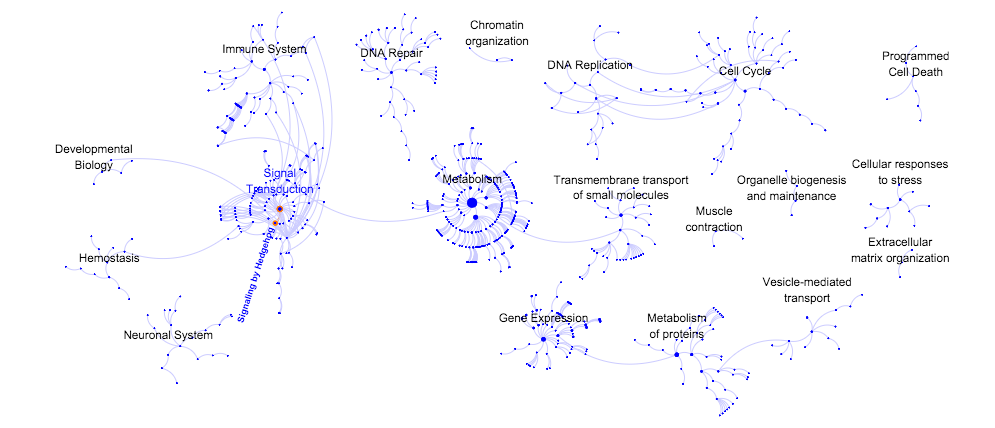
\includegraphics[width=\textwidth]{at_interactome}
  \caption[\textit{Arabidopsis thaliana} interactome]{The entire \textit{A. thaliana}  interactome, as displayed by the Reacome interactive pathway browser. This interactome is comparably dense to the human interactome seen in \ref{fig:human_interactome}, which makes it a better candidate for running network algorithms.}
  \label{fig:at_interactome}
  \end{center}
\end{figure}

Our ability to look at the entire interactome of species such as \textit{A. thaliana} allows us to investigate some of the global effects of genetic manipulation on signal transduction. This is especially useful in model organisms like \textit{A. thaliana}, since we can actually perform genetic manipulations on them quickly, safely, and ethically, unlike with human beings. Additionally, our ability to breed model organisms in the lab means that we can use specific datasets with large sample sizes. This is very useful compared to human datasets, which are generally based on small sample sizes, since human gene expression data is generally collected from pseudo-random, sparse cases when a person has a degenerate tissue type, such as a tumor, rather than under direct experimental manipulation.\par

\section{\new{Transition}{Not sure if this should be its own section or if it will be incorporated into the previous.}}

\new{Put in transition.}{Transitions are good.}

\chapter{Hypergraphs \& Hyperpaths}

\new{In order to model cell signaling pathways computationally, it is first necessary to choose the correct computational object to represent our data. For this, we can use graphs, but there are some ways in which graphs are not the ideal structure, and leave some things to be desired (see Figure \ref{fig:anna_fig}). Instead of using graphs, we will define a generalization of a directed graph, called a directed hypergraph, and use it to model cell signaling pathways and PPI networks.}{Intro}

\begin{figure}[h]
  \begin{center}
    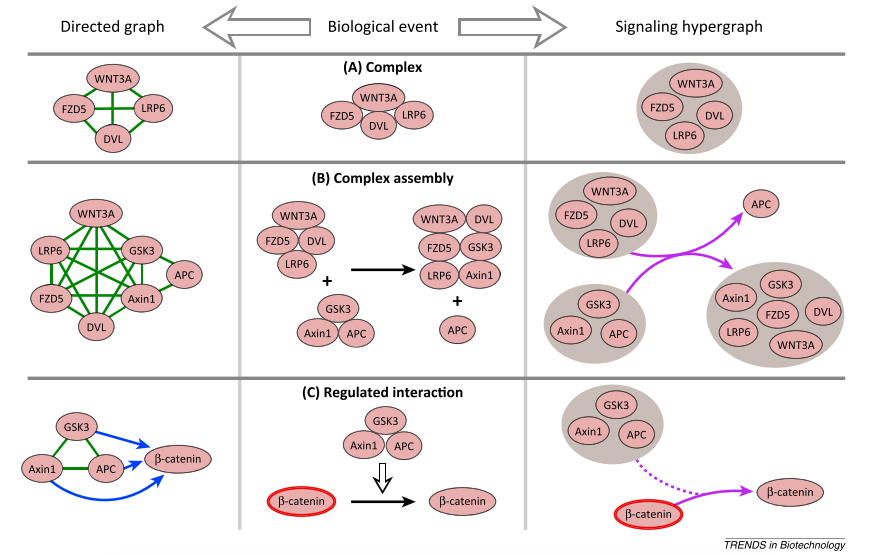
\includegraphics[width=\textwidth]{anna_fig}
  \caption[The issue with standard graphs.]{CAPTION AND CITATION}
  \label{fig:anna_fig}
  \end{center}
\end{figure}

\section{Graphs and their Limitations}

While standard\footnote{The term ``standard" is used to describe traditional graphs, since the terms ``regular" and ``normal," both refer to specific types of graphs.} graphs are useful for many applications, they are severely limited in their ability to represent cell-signaling interactions.  Since they can only show pairwise interactions between nodes, whenever there is an interaction that requires more than two connections, the visualization of the graph becomes confusing, and biologically meaningless.  Furthermore, interactions involving multiple molecules require an enormous amount of different edges to represent all of the sub-interactions that take place.  Determining whether two edges are part of the same biological event is a non-trivial problem, and requires manual curation to solve, at this time.\par

\begin{figure}[thbp]
  \begin{center}
    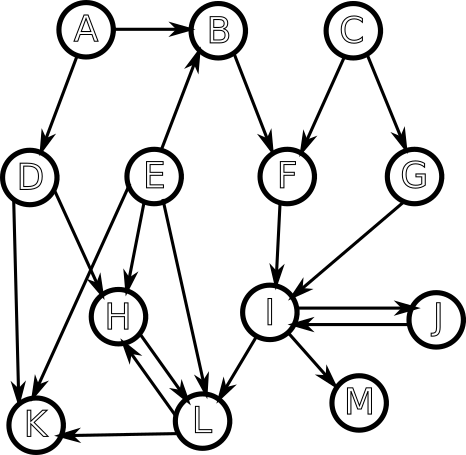
\includegraphics{example-standard-graph}
  \caption[A standard graph]{An example of a standard graph. All edges represent directed, pairwise interactions between two nodes. Biologically, it is difficult to extract meaningful signaling pathway information from this graph, since protein complex formation and degradation is ambiguous.}
  \label{fig:example-standard-graph}
  \end{center}
\end{figure}

One area of cell-signaling that becomes particularly problematic in standard graphs is the formation, interaction, and destruction of protein complexes.  The easiest way that complexes can be represented in standard graphs is by creating a complete subgraph of all of the elements of the protein complex.  On their own, these complete subgraphs can yield useful information about the make-up of a protein complex, but once they begin interacting with other elements of the graph, the graph becomes much more complex, as all of the proteins in the complex must be represented independently.  In the case of interactions between multiple large complexes, it becomes the case that the standard graph representation of this interaction is a large complete subgraph that contains nodes for all of the proteins involved in either complex.  It is then computationally impossible to distinguish whether the entity being described by the subgraph is the interaction between multiple protein complexes, or simply one large complex that contains all of the components of both complexes.  Furthermore, since the complete subgraphs which represent complexes are undirected, it is extremely difficult to tell what the inputs or outputs of a biochemical reaction may be.\par

Another shortcoming of standard graphs in representing complex biological interactions is that there is no way in which to represent positive or negative regulation of interactions.  Since there is a standardized way in which edges interact with nodes, there is no way to differentiate types of interactions between nodes.  This poses a challenge when there are regulators or catalysts present that are necessary for a reaction, but are not part of the inputs or outputs of the reaction.  If regulators are to be included in a standard graph representation of a cell-signaling network, they become indistinguishable from any other types of interactions that are taking place.  This lack of specificity is problematic, as it treats all interactions as equal, and hides potentially useful information from the graph\footnote{\new{The Reacome database is available for download as a standard graph, but it is not available as a directed graph. This means that we could not use their graphs as a standard graph comparison to ours.}{Anna}}.\par

To resolve the issues presented by standard graphs, we instead use a generalization called a \textit{hypergraph} that allows for the addition of more detail  and specificity within the data structure than standard graphs allow.  In particular, hypergraphs allow for both the representation of protein complexes in the form of \textit{hypernodes}, which we think of simply as a set of one or more nodes, and for the representation of complex, directed interactions that can have multiple inputs and outputs.  We represent these interactions with the use of \textit{hyperedges}, which define a set of one or more hypernodes.  Since a hyperedge may include more than two hypernodes, we gain the ability to represent both multi-protein interactions, as well as to define the notions of regulation on reactions.\par

\section{Hypergraphs}

\begin{figure}[thbp]
  \begin{center}
    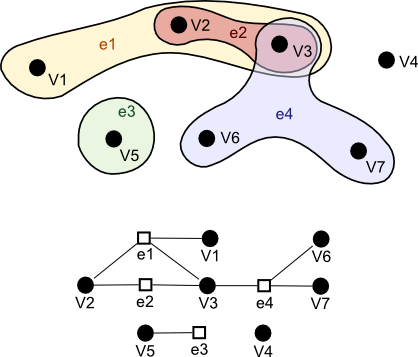
\includegraphics[width=\textwidth/2]{undirected_hypergraph}
  \caption[An example undirected hypergraph]{\new{An example of an undirected hypergraph (\cite{sharpen}), where each edge is shown by a colored region, as well as the conversion of the hypergraph to a standard graph.}{I could also draw this on my own, I suppose.}}
  \label{fig:undirected_hypergraph}
  \end{center}
\end{figure}

Where a directed graph represents directed, pairwise interactions between only two vertices, we can use \textit{directed hypergraph} to represent directed interactions between sets of vertices (nodes). We formally define a directed hypergraph, $\mathcal{H}$, as a pair $(V,E)$, where $V$ is a finite set of vertices and $E \subseteq 2^V \times 2^V$ is a finite set of \textit{directed hyperedges} connecting members of $V$ such that, for every $e=(T(e),H(e)) \in E$, $T(e) \cap H(e) = \emptyset$, and $T(e)$, $H(e) \neq \emptyset$.  We refer to $T(e)$ as the \textit{tail} of the hyperedge, and to $H(e)$ as the \textit{head} of the hyperedge.\par

\begin{figure}[thbp]
  \begin{center}
    \includegraphics{example-hypergraph}
  \caption[An example directed hypergraph]{An example of the hypergraph, $\mathcal{H}=(V,E)$ that corresponds to the standard graph shown in Figure \ref{fig:example-standard-graph}. Note that each edge now contains more specific information about the propogation of a signal through the network. For this example, $V={A,B,...,M}$ and each hyperedge is shown by a compund arrow, for example the edge whose tail is hypernodenode $A$ and whose tail is hypernodes $B$ and $D$.}
  \label{fig:example-hypergraph}
  \end{center}
\end{figure}

It is important to note that a standard directed graph is a special case of a directed hypergraph.  This is the case if every hypernode in the graph contains only one element, and if each edge has exactly one head element, and one tail element.  This has two important implications for algorithms that run on directed hypergraphs.  First, this means that there is no loss in functionality caused by using a hypergraph representation of a cell network, since anything that could be computed on a standard directed graph can be recreated exactly using the special case of the hypergraph. Secondly, this is important, because it means that anything that can be computed on a standard graph will be at least as computationally difficult to compute when generalized to a hypergraph.  In fact, we find that many tasks that are computationally easy on standard graphs become very difficult when generalized to hypergraphs (\cite{Ritz2014a}).\par

\begin{figure}[thbp]
  \begin{center}
    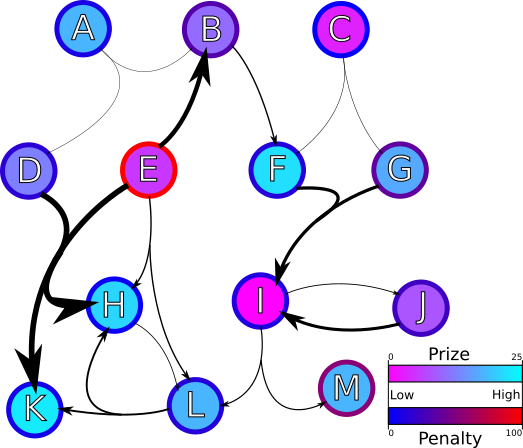
\includegraphics{example-hypergraph-weighted}
  \caption[A weighted hypergraph]{The same hypergraph as in \ref{fig:example-hypergraph}, now weighted with node prizes (inner color) and dangling penalties (outer color). Edge thickness corresponds with edge weight. Intuitively, to find the PCSHS for this hypergraph, we want to find the subnetwork that maximizes the amount of blue, and minimizes the amount of both red nodes and thick lines.}
  \label{fig:example-hypergraph-weighted}
  \end{center}
\end{figure}

\section{Hyperpaths \& Connectivity\new{consider revising this using earlier defs}[yup]}
In order to find the shortest route between two vertices, in a directed hypergraph, we define the notion of a \textit{hyperpath}, $P$, on the directed hypergraph $\mathcal{H}$.  We think of $P(s,t)$ as the list of vertices and hyperedges that one must pass through in order to traverse through the directed hypergraph from vertex $s$ to $t$. The existence of a hyperpath between two nodes encodes the notion of ``connectivity" between those nodes.  If a hyperpath exists between nodes $s$ and $t$, we say that they are \textit{connected}. Furthermore, given some root hypernode, $u$, we refer to the set of all nodes, $V$ in a hypergraph for which there exists some $P(u,v)$ (where $v \in V$) as a \textit{hypertree}. This is a useful definition, because it allows us the notion of a \textit{connected hypergraph}, a hypergraph in which every node is connected by some hyperpath to every other node in the hypergraph.\par

\subsection{Directed Hyperpaths}

There are many ways in which we can define hyperpaths, but for the purposes of finding Steiner Trees in directed hypergraphs, we must define a simple \textit{directed hyperpath} between nodes $s$ and $t$. We can think of a directed hyperpath $P(s,t)=\{s,e_2,v_3,...,e_{n-1},t\}$ as an ordered list of nodes and edges, beginning with $s$ and ending with $t$ such that for any edge, $e_i$, in the path, $v_{i-1}$ is in the tail of $e_i$, and $v_{i+1}$ is in the head of $e_i$.\par

\chapter{Prize Collecting Steiner Hypershrubs}

In order for us define and develop a Prize-Collecting Steiner Hyptershrub, we begin by formulating the notion of a \textit{Steiner Hypershrub}. This allows us to develop an implementation that where some nodes, referred to as our \textit{target set}, are included in the solution, by definition. We begin like this to make the development and debugging of the ILP slightly easier, since it allows us to work from the target set to other nearby nodes, instead of forcing the ILP to discover every node that it needs to include.\par

\new{
We now can define the Prize-Collecting Steiner Hypershrub (PCSHS), $\mathcal{S} = (V^\prime,E^\prime)$, to be the set of hypernodes and hyperedges for which total vertex prizes are maximized, and total edge weights (and dangling penalties) are minimized. Due to the structure of hypergraphs, rather than formulating a generalization of a single-source tree, as is used in standard graphs, we will instead construct a \textit{hypershrub}, as a structure that can contain multiple sources, and multiple targets. At this point, it is necessary for us to define two classes of nodes that may be present in a PCSHS: root nodes and leaf nodes.  We say a node is a \textit{root} if it is present in a PCSHS and does not have any incoming hyperedge in the PCSHS (that is, it is not in the tail of any edge in the hypergraph). We can define a root node, $d$ as any node such $d \in V^\prime$ and $d \notin T(e)$ for all $e \in \mathcal{S}$. Similarly, we say a node is a \textit{leaf} if it is present in a PCSHS, and not in the head of any edge in the hypergraph. A leaf, $c$, is defined as any node $l \in V^\prime$ and $l \notin T(e)$ for all $e \in \mathcal{S}$.\par
We now formulate the decision problem as follows:\par
\paragraph{Steiner Hypershrub.}Given a hypergraph $\mathcal{H}$, with vertices $V$ and hyperedges $E$ and some set of hyperedges $A \subseteq E$. From this, we define:\par
\begin{equation}
  H(A) = \bigcup_{e \in A} H(e)
\end{equation}
and
\begin{equation}
  T(A) = \bigcup_{e \in A} T(e)
\end{equation}
From this, we can also define the induced subset of nodes $V(A) = H(A) \cup T(A)$. From this, we also define the set of everything that is in the tail of some edge, but not in the heads of any hyperedges in $A$ as $D(A) = V(A) \setminus H(A)$. The set $D(A)$ represents the set of the induced roots from $A$. Similarly, we find the induced leaves from $A$ by defining $C(A) = V(A) \setminus T(A)$. From these definitions, we can construct three definitions of Steiner Hypershrubs, \textit{B-Steiner Hypershrubs}, \textit{F-Steiner Hypershrubs}, and \textit{BF-Steiner Hypershrubs}. For all three of the Steiner Hypertrees, we begin with a hypergraph, $\mathcal{S}$, and two sets of nodes: a source set, $S$, and a sink set, $T$, where $S,T \subseteq V$. We now define:\par
\paragraph{B-Steiner Hypershrub.}Given a hypergraph $\mathcal{H}$ and node sets $S$ and $T$ we that there is a B-Steiner Hypershrub, $\mathcal{S}^{\prime}$ if there exists some subset of hyperedges $A$ such that:
\begin{equation*}
  C(A) \subseteq T
\end{equation*}
and
\begin{equation*}
  D(A) = S
\end{equation*}
We call the induced hypergraph of $A$ the B-Steiner Hypershrub, $\mathcal{S}^{\prime}$.\par
\paragraph{F-Steiner Hypershrub.}Given a hypergraph $\mathcal{H}$ and node sets $S$ and $T$ we that there is a F-Steiner Hypershrub, $\mathcal{S}^{\prime\prime}$ if there exists some subset of hyperedges $A$ such that:
\begin{equation*}
  C(A) = T
\end{equation*}
and
\begin{equation*}
  D(A) \subseteq S
\end{equation*}
We call the induced hypergraph of $A$ the F-Steiner Hypershrub, $\mathcal{S}^{\prime\prime}$.\par
\paragraph{BF-Steiner Hypershrub.}Given a hypergraph $\mathcal{H}$ and node sets $S$ and $T$ we that there is a BF-Steiner Hypershrub, $\mathcal{S}^{\prime\prime\prime}$ if there exists some subset of hyperedges $A$ such that:
\begin{equation*}
  C(A) = T
\end{equation*}
and
\begin{equation*}
  D(A) = S
\end{equation*}
We call the induced hypergraph of $A$ the BF-Steiner Hypershrub, $\mathcal{S}^{\prime\prime\prime}$.\par

}{Jim, please double check this if you can.}

\section{Definition of PCSHS}

To make our Prize-Collecting Steiner Hypershrub, $\mathcal{S}$, we begin with a ``parent" hypergraph, $\mathcal{H} = (V,E)$, and a set of target nodes, $T$, such that $T \subseteq V$.  We refer to each hypernode as some $x$ such that $x \in V$\footnote{We use ``$x$" as an element of $V$, rather than lowercase ``$v$" to avoid the visual confusion between lowercase $v$ and uppercase $V$}, and each edge is some $e$ such that $e \in E$.  When building $\mathcal{H}$, we initially seed the hypergraph.  Each hyperedge is assigned a weight, that is, a cost associated with including that edge in the solution hypergraph, $\mathcal{S}$.  We then assign each hypernode in $\mathcal{H}$ two values, a prize for being included in $\mathcal{S}$, as well as a penalty associated with being a \textit{root} hypernode.\par
\section{Prize-Collecting Steiner Hypershrub ILP}

To solve for solutions to the Prize-Collecting Steiner Hypershrub

Given an input hypergraph $\mathcal{H}=(V,E)$, and a set of target nodes, $T$, we construct a Steiner Hypershrub, (DEFINE) $\mathcal{S}= (V^\prime,E^\prime)$, where $V^\prime \subseteq V$ and $E^\prime \subseteq E$.  We build $\mathcal{S}$ using an ILP which encodes the definition of a Steiner Hypershrub.  In order to accomplish this, we define three indicator variables, $\alpha_v$, $\alpha_e$, and $\delta_v$, where $v$ and $e$ are hypernodes or hyperedges in $\mathcal{H}$.  If hypernode $x$ is in the solution of the ILP, $\alpha_v$ will have a value of 1, otherwise it will be equal to 0.  Similarly, if edge $e$ is present in the solution, $\alpha_e$ will take a value of 1. The value of $\delta_v$ will be determined by whether a hypernode is dangling.\par

We find the Steiner Hypershrub $\mathcal{S}$ by optimizing the function:

\begin{equation} \label{eq:ilpsum}
 \argmax_{\alpha, \delta} \sum_{v \in V} g_v \alpha_v - \sum_{e \in E} c_e \alpha_e - \sum_{v \in V} h_v \delta_v
\end{equation}

Subject to the set of linear constraints:

\begin{align}
 \alpha_v \geq 1 \qquad\qquad &\forall\; v \in T\label{eq:ilpT}\\
 \sum_{v \in H(e)} \alpha_v \geq \lvert H(e)\rvert \alpha_e \qquad\qquad &\forall\; e \in E\label{eq:ilpinchead}\\
 \sum_{v \in T(e)} \alpha_v \geq \lvert T(e)\rvert \alpha_e\qquad\qquad &\forall\; e \in E\label{eq:ilpinctail}\\
 \delta_v \leq \alpha_v \qquad\qquad &\forall\; v \in V\label{eq:ilpdang1}\\
 \delta_v \geq \alpha_{v} - \sum_{e:v \in H(e)} \alpha_e \qquad\qquad &\forall\; v \in V\label{eq:ilpdang2}\\
0 \leq \delta_v \leq 1 \qquad\qquad &\forall\; v \in V\label{eq:ilpdang3}%
\end{align}%


Here, the objective function \eqref{eq:ilpsum} tries combinations of nodes ($\alpha_v$), edges ($\alpha_e$), and dangling nodes ($\delta_v$) that maximize the sums of node prizes ($g_v$), minimize the sums of edge costs ($c_e$), and minimize the sums of dangling penalties ($h_v$). Constraint \eqref{eq:ilpT} encodes that every target node in $T$ is in the solution, $\mathcal{S}$.  Constraints \eqref{eq:ilpinchead} and \eqref{eq:ilpinctail} ensure that if an edge is in $\mathcal{S}$, any nodes incident on that edge (i.e. in the head or tail of that edge) will also be in $\mathcal{S}$.  Finally, constraints \eqref{eq:ilpdang1}, \eqref{eq:ilpdang2}, and \eqref{eq:ilpdang3} encode the ability for nodes to dangle if they do not have an incoming edge. To illustrate what each of these constraints does in more detail, we will construct a simple example, and examine each constraint within that example.\par

\begin{figure}[th]
  \begin{minipage}[b]{0.30\linewidth}
    \centering
    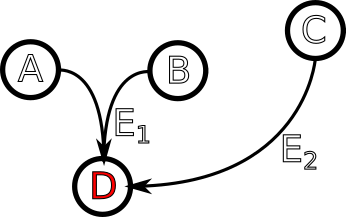
\includegraphics[width=\linewidth]{dummy-before}
    \par\vspace{0pt}
  \end{minipage}%
  \begin{minipage}[b]{0.30\linewidth}
    \centering%
    \begin{tabular}{ |l|l|l| }%
      \hline%
      \multicolumn{3}{|c|}{Nodes} \\%
      \hline \hline
      Node & $g_v$ &  $h_v$ \\ \hline%
      $A$ & 10 &  1\\ \hline%
      $B$ & 10 &  1\\ \hline%
      $C$ & 1 &  10\\ \hline%
      $D$ & 10 &  10\\ \hline%
    \end{tabular}%
    \par\vspace{0pt}
  \end{minipage}
  \begin{minipage}[b]{0.30\linewidth}
    \centering%
    \begin{tabular}{ |l|l| }%
      \hline%
      \multicolumn{2}{|c|}{Edges} \\%
      \hline \hline
      Edge & $c_e$ \\ \hline%
      $E_1$ & 1 \\ \hline%
      $E_2$ & 10 \\ \hline%
    \end{tabular}%
    \par\vspace{0pt}
  \end{minipage}
\caption[A small hypergraph, with node and edge data]{A simple hypergraph, and its associated node and edge weights.}
\label{fig:dummy-before}
\end{figure}

\paragraph{Example.}Consider the hypergraph shown in Figure \ref{fig:dummy-before}. For this hypergraph, the PCSHS that comes from this graph should consist of hypernodes $A$, $B$, and $D$, as well as hyperedge $E_1$. This is obvious, since nodes $A$ and $B$, which will be dangling in the solution, both have low dangling penalties and high prizes, while node $C$ has a very large dangling penalty relative to its prize. Similarly, $E_1$ has a relatively low cost, whereas $E_2$ has a very high cost. Finally, $D$ is considered a target, in this case, and is therefore automatically included in the solution. Knowing what the solution should be, we can use this hypergraph to demonstrate the effect of each linear constraint in our ILP.\par

\begin{table}[!h]
\begin{center}
  \label{tab:obj_values_dummy}
  \caption[Objective values of dummy hypergraph.]{\new{All of the possible solutions that satisfy all necessary linear constraints, and their corresponding objective values. We see that the induced subgraph (DEFINE) from $E_1$ yields the optimal solution.}{Added to show all ``legal" solutions, and what obj. value they yield.}}
\begin{tabular}{ |l|l|l| }%
  \hline%
  \multicolumn{3}{|c|}{Subgraphs (caption doesn't work plz someone help)} \\%
  \hline \hline
  $V$ & $E$ & Objective Value \\ \hline%
  $A,B,D$ & $E_1$ & 27 \\ \hline%
  $C,D$ & $E_2$ & -9 \\ \hline%
  $A,B,C,D$ & $E_1,E_2$ & -2 \\ \hline%
\end{tabular}%
\end{center}
\end{table}

We now know that, for the optimal PCSHS, $\alpha_A$, $\alpha_B$, $\alpha_D$, and $\alpha_{E_1}$ are all equal to 1 (that is, they are included in the solution), and $\alpha_C$ and $\alpha_{E_2}$ are equal 0. Additionally, we know that in this solution $A$ and $B$ are dangling nodes, therefore $\delta_A$ and $\delta_B$ are both 1, and $\delta_C$ and $\delta_D$ are both 0. Finally, we are given that $D$ is a target node, hence $T=\{D\}$.\par

First let us look at the objective function, Formula \eqref{eq:ilpsum}. We can call each of the three sums included the equation which calculate the total node prizes, edge costs, and dangling penalties $\Xi$, $\Phi$, and $\Psi$, respectively. Given the values of $\alpha_v$, $\alpha_e$, and $\delta_v$ that we know should yield the PCSHS, we get find:
\begin{gather*}
 \Xi = 30\\
 \Phi = 1\\
 \Psi = 2\\
 \implies \Xi - \Phi - \Psi = 27\\
\end{gather*}%
If $C$ or $E_2$ were to be added, or any node or edge were removed from the PCSHS, the total value of the objective function would decrease, therefore yielding a suboptimal solution to the ILP.\par

Now, we can begin to look at how each linear constraint governs the behavior of the ILP. Let's begin with constraint \eqref{eq:ilpT}. For our hypergraph, $T$ only has one element, $D$, constraint \eqref{eq:ilpT} only needs to be checked for one node. We know that $\alpha_D = 1$, therefore constraint \eqref{eq:ilpT} simplifies to:
\begin{align*}
  \alpha_D &\geq 1\\
\end{align*}
We see that constraint \eqref{eq:ilpT} holds for all $v$ in $T$, therefore we know that all members of the target set are included in the PCSHS.\par

Next, we can look at constraints \eqref{eq:ilpinchead} and \eqref{eq:ilpinctail}. Since these constraints are the same, except for whether they are concerned with the head or tail of a hyperedge, we can evaluate the effect of only constraint \eqref{eq:ilpinchead}, and assume that constraint \eqref{eq:ilpinctail} works in the same way. To assess this constraint, we must see how if the inequality holds for all edges in the hypergraph. We begin by looking at $E_1$. We know that $H({E_1})=D$, and that $\lvert H(e) \rvert = 1$, therefore we can check:
\begin{align*}
  \alpha_D &\geq 1 \bullet \alpha_{E_1}\\
\end{align*}%
So, we see that constraint \eqref{eq:ilpinchead} holds for $E_1$. Now, we can check for $E_2$ (whose head is also only $D$):
\begin{align*}
  \alpha_D &\geq 1 \bullet \alpha{E_2}\\
\end{align*}%
We see that this inequality also holds. This means that, since the inequality holds for all hyperedges, that for every edge in the hypergraph, its head is also included in the hypergraph. We can easily extend this to see that \eqref{eq:ilpinctail} enforces the same for the tails of every hyperedge.\par

Finally, we can look at the three constraints that allow hypernodes to be dangling: constraints \eqref{eq:ilpdang1}, \eqref{eq:ilpdang2}, and \eqref{eq:ilpdang3}. First, we look at constraint \eqref{eq:ilpdang1} \emph{I need to figure out the proper way to align these.}:
\begin{alignat*}{4}
  \delta_A &\leq \alpha_A \qquad \delta_B &&\leq \alpha_B \qquad \delta_C &&\leq \alpha_C \qquad \delta_D &&\leq \alpha_D\\
\end{alignat*}
Now, we see that constraint \eqref{eq:ilpdang1} holds for all nodes in the PCSHS. \emph{I will get the other two constraints up soon.}\par

\section{Roots and Leaves Problem}

When we implement the ILP in a more complex hypergraph, such as the hypergraph shown in Figure \ref{fig:example-hypergraph-weighted}, we find that it creates a hypergraph that consists of multiple smaller hypergraphs (Figure \ref{fig:example-hypergraph-weighted-after-ILP}), rather than a continuous subnetwork. Our original implementation ends up returning a group of disconnected hypergraphs that represent regions with high prize to edge/dangling cost ratios, separated by gaps where the parent hypergraph had regions of low prize to edge/dangling cost ratios. While this result is intersting in itself, it will not necessarily create a soltion that is biologically interesting, once we begin looking for PCSHSs in pathway signaling data.\par

\begin{figure}[th]
  \begin{center}
    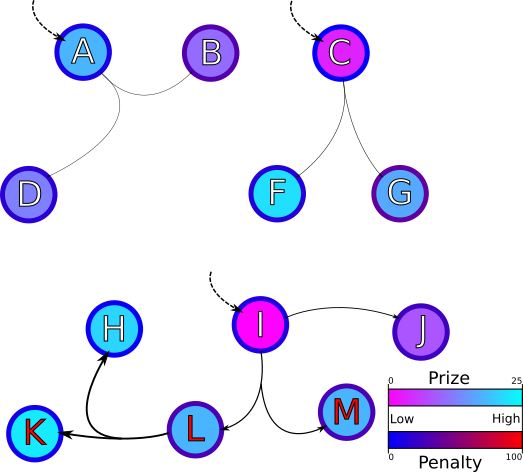
\includegraphics{example-hypergraph-weighted-after-ILP}
  \caption[Output from ILP with disconnected sub-hypergraphs]{The output of our ILP, when it is run on the hypergraph shown in Figure \ref{fig:example-hypergraph-weighted}. The dashed arrows indicate a dangling hypernode.}
  \label{fig:example-hypergraph-weighted-after-ILP}
  \end{center}
\end{figure}

To fix this problem, we must incorporate the notion of hyperpaths and connectedness to our implementation of the PCSHS, as well as define the class of leaf variables in our formulation. Additionally, we must construct a matrix\footnote{Actually implemented as a Python dictionary, if that matters.} of whether or not there exists a hyperpath between every pair of nodes in $\mathcal{H}$. As such, we adopt the notation $\iota_x$, as a binary variable that indicates whether node $x$ is a leaf in the solution.

\chapter{Methods and Results}

  \section{Network Construction and Weighting}
  In order to construct directed signaling hypergraphs of biological pathways, we use pathway data from preexisting, curated protein-protein interaction networks, available publically. For this, pathway signaling information was downloaded from the curated Reactome pathway database (\cite{Croft2014}, \cite{Milacic2012}), and parsed using a Java script (\cite{AnnaCorrespondence}) into two flat files containing node and edge information necessary to construct the hypergraph (See Appendix B).\par
  The networks generated from the Reactome database specify each hypernode as a combination of one or more proteins or small molecules. For simplicity, each hypernode was ``converted" into a regular node for the purpose of algorithm implementation, and the components' information was saved so that they could be reconstructed \textit{post hoc}. Additionally, each hyperedge contained information about whether the reaction that it represented was regulated either positively or negatively by one or more nodes. Positive regulators were added to the tail of their respective hypernodes, since they are assumed to be necessary reactants for the edge, and should therefore be considered part of the signaling network. Negative regulators, on the other hand, were excluded from the flat files, since the way that they act on reactions poses an interesting problem in modeling, since the current definition of PCSHS assumes that all node prizes and edge weights are positive (see Future Directions).\par
  \new{From the edge files, hypergraphs were constructed using the Hypergraph Algorithms Package (HALP, \cite{halp}). Edge files gave enough information to create induced hypergraphs, which were then weighted based on information stored in node files. For the implementation PCSHS to create meaninful subnetworks, it is important that the parent hypergraph have a meaningful, biologically informed weighting scheme applied. However, it is often the case that data are difficult to acquire and add to the hypergraph, so simple default settings were first applied to each parameter. By default, each node was given a prize of 1, and a dangling penalty of 5.  Additionally, each edge was given a default weight of 1, so that the algorithm would try to minimize the number of edges.}{Methods section.}

  \section{Simulated Data}

  To assess the efficacy of this ILP in generating the correct Prize Collecting Steiner Hypershrub, it is first necessary to perform a series of benchmarking tests on known datasets and hypergraphs.  This will allow us to determine if the algorithm is performing as expected, and generating results that can be corroborated manually.\par

  \subsection{Simple Example Hypergraphs}

  \subsection{Potential Special Cases}

  \section{PCSHS in Real Data}

   \subsection{Human Cancer Data}

  \section{Comparison to Standard Graphs}

  \emph{Make python file to convert to standard graphs!}

  \new{To test how well this algorithm is able to construct sub-hypergraphs that are more meaningful than their standard counterparts, we look at the same implementation on hypergraphs that have been converted to standard graphs. For this conversion, each hyperedge in the original hypergraph was replaced with a set of directed edges that corresponded to \emph{FINISH THIS \P}}{}

\chapter{Future Directions}
 \begin{itemize}
   \item{Heat mapping to weight hypergraphs (Random walks).}
   \item{Computation of individual or multiple subnetworks.}
 \end{itemize}

 \section{\new{Complexed Hypergraphs}{Reordering}}

 \new{
 We can define sets of two or more nodes as a hypernode, which are members of the power set of $V$.  These can be incorporated into a directed hypergraph to form a \textit{complexed directed hypergraph}.  We define a \textit{complexed directed hypergraph}, $\mathcal{H}$, as the triple $(V,U,E)$ in which $V$ is a finite set of vertices, $U \subseteq 2^V$ is a finite set of hypernodes, and $E \subseteq 2^U \times 2^U$ is a finite set of hyperedges such that, for every $e=(T(e),H(e)) \in E$, $T(e) \cap H(e) = \emptyset$ and $T(e)$, $H(e) \neq \emptyset$.\par}{Reordering}

\chapter*{Conclusion}
         \addcontentsline{toc}{chapter}{Conclusion}
	\chaptermark{Conclusion}
	\markboth{Conclusion}{Conclusion}
	\setcounter{chapter}{4}
	\setcounter{section}{0}

Here's a conclusion, demonstrating the use of all that manual incrementing and table of contents adding that has to happen if you use the starred form of the chapter command. The deal is, the chapter command in \LaTeX\ does a lot of things: it increments the chapter counter, it resets the section counter to zero, it puts the name of the chapter into the table of contents and the running headers, and probably some other stuff.

So, if you remove all that stuff because you don't like it to say ``Chapter 4: Conclusion'', then you have to manually add all the things \LaTeX\ would normally do for you. Maybe someday we'll write a new chapter macro that doesn't add ``Chapter X'' to the beginning of every chapter title.

\section{More info}
And here's some other random info: the first paragraph after a chapter title or section head \emph{shouldn't be} indented, because indents are to tell the reader that you're starting a new paragraph. Since that's obvious after a chapter or section title, proper typesetting doesn't add an indent there.


%If you feel it necessary to include an appendix, it goes here.
    \appendix
      \chapter{Benchmarking Graphs \& Supplemental Data}

      \chapter{Algorithms \& Programs}

        \paragraph{Construction of LP files.}The constructor \verb|build_lp.py| builds a \texttt{.lp} file that can be optimized by the ILP solver CPLEX. The constructor takes the following files as arguments, as well as a column delimeter (default ``\texttt{;}") and a node delimeter (default ``\texttt{,}").

        Edge file (\texttt{ex-edges.txt}):\\
        \rule{\textwidth}{1pt}
        \verbatiminput{../examples/ex-edges.txt}
        \rule{\textwidth}{1pt}

        \newpage

        Node file (\texttt{ex-nodes.txt}):\\
        \rule{\textwidth}{1pt}
        \verbatiminput{../examples/ex-nodes.txt}
        \rule{\textwidth}{1pt}

        \newpage

        Output file (\texttt{ex.lp}):\\
        \rule{\textwidth}{1pt}
        \begin{lstlisting}
Maximize
 obj: 2.0 Kx + 8.0 Gx + 16.0 Jx + 4.0 Hx + 7.0 Ax + 12.0 Dx + 7.0 Lx + 14.0 Bx + 7.0 Mx + 3.0 Fx + 24.0 Ix + 21.0 Cx + 19.0 Ex - 0.0 Kd - 37.0 Gd - 24.0 Jd - 4.0 Hd - 10.0 Ad - 16.0 Dd - 0.0 Ld - 32.0 Bd - 0.0 Md - 14.0 Fd - 12.0 Id - 1.0 Cd - 98.0 Ed - 31.0 hyperedge8 - 5.0 hyperedge3 - 45.0 hyperedge12 - 33.0 hyperedge6 - 14.0 hyperedge2 - 4.0 hyperedge1 - 12.0 hyperedge10 - 9.0 hyperedge7 - 14.0 hyperedge5 - 57.0 hyperedge4 - 19.0 hyperedge11 - 8.0 hyperedge9
Subject To
 c44_hyperedge8: Jx - 1 hyperedge8 >= 0
 c43_hyperedge8: Ix - 1 hyperedge8 >= 0
 c44_hyperedge3: Cx - 1 hyperedge3 >= 0
 c43_hyperedge3: Fx + Gx - 2 hyperedge3 >= 0
 c44_hyperedge12: Ex - 1 hyperedge12 >= 0
 c43_hyperedge12: Bx - 1 hyperedge12 >= 0
 c44_hyperedge6: Fx + Gx - 2 hyperedge6 >= 0
 c43_hyperedge6: Ix - 1 hyperedge6 >= 0
 c44_hyperedge2: Bx - 1 hyperedge2 >= 0
 c43_hyperedge2: Fx - 1 hyperedge2 >= 0
 c44_hyperedge1: Ax - 1 hyperedge1 >= 0
 c43_hyperedge1: Dx + Bx - 2 hyperedge1 >= 0
 c44_hyperedge10: Ix - 1 hyperedge10 >= 0
 c43_hyperedge10: Lx + Mx - 2 hyperedge10 >= 0
 c44_hyperedge7: Ix - 1 hyperedge7 >= 0
 c43_hyperedge7: Jx - 1 hyperedge7 >= 0
 c44_hyperedge5: Ex - 1 hyperedge5 >= 0
 c43_hyperedge5: Hx + Lx - 2 hyperedge5 >= 0
 c44_hyperedge4: Dx + Ex - 2 hyperedge4 >= 0
 c43_hyperedge4: Hx + Kx - 2 hyperedge4 >= 0
 c44_hyperedge11: Lx - 1 hyperedge11 >= 0
 c43_hyperedge11: Hx + Kx - 2 hyperedge11 >= 0
 c44_hyperedge9: Hx - 1 hyperedge9 >= 0
 c43_hyperedge9: Lx - 1 hyperedge9 >= 0
 c45_A: Ad - Ax <= 0
 c45_B: Bd - Bx <= 0
 c45_C: Cd - Cx <= 0
 c45_D: Dd - Dx <= 0
 c45_E: Ed - Ex <= 0
 c45_F: Fd - Fx <= 0
 c45_G: Gd - Gx <= 0
 c45_H: Hd - Hx <= 0
 c45_I: Id - Ix <= 0
 c45_J: Jd - Jx <= 0
 c45_K: Kd - Kx <= 0
 c45_L: Ld - Lx <= 0
 c45_M: Md - Mx <= 0
 c46_K: Kd - Kx + hyperedge11 + hyperedge4 >= 0
 c46_G: Gd - Gx + hyperedge3 >= 0
 c46_J: Jd - Jx + hyperedge7 >= 0
 c46_H: Hd - Hx + hyperedge5 + hyperedge11 + hyperedge4 >= 0
 c46_A: Ad - Ax >= 0
 c46_D: Dd - Dx + hyperedge1 >= 0
 c46_L: Ld - Lx + hyperedge5 + hyperedge10 + hyperedge9 >= 0
 c46_B: Bd - Bx + hyperedge1 + hyperedge12 >= 0
 c46_M: Md - Mx + hyperedge10 >= 0
 c46_F: Fd - Fx + hyperedge2 + hyperedge3 >= 0
 c46_I: Id - Ix + hyperedge6 + hyperedge8 >= 0
 c46_C: Cd - Cx >= 0
 c46_E: Ed - Ex >= 0
Bounds
 Kx = 1
 Kd = 0
 Lx = 1
 Ld = 0
 Mx = 1
 Md = 0
Binary
 Ax
 Bx
 Cx
 Dx
 Ex
 Fx
 Gx
 Hx
 Ix
 Jx
 Kx
 Lx
 Mx
 Ad
 Bd
 Cd
 Dd
 Ed
 Fd
 Gd
 Hd
 Id
 Jd
 Kd
 Ld
 Md
 hyperedge1
 hyperedge10
 hyperedge11
 hyperedge12
 hyperedge2
 hyperedge3
 hyperedge4
 hyperedge5
 hyperedge6
 hyperedge7
 hyperedge8
 hyperedge9
End

        \end{lstlisting}
        \rule{\textwidth}{1pt}

      \chapter{Biological Data}

      \chapter{Version Information}

      This appendix will be concerned with which versions of various softwares I used.


%This is where endnotes are supposed to go, if you have them.
%I have no idea how endnotes work with LaTeX.

  \backmatter % backmatter makes the index and bibliography appear properly in the t.o.c...

% if you're using bibtex, the next line forces every entry in the bibtex file to be included
% in your bibliography, regardless of whether or not you've cited it in the thesis.
    \nocite{*}

% Rename my bibliography to be called "Works Cited" and not "References" or ``Bibliography''
% \renewcommand{\bibname}{Works Cited}

%    \bibliographystyle{bsts/mla-good} % there are a variety of styles available;
%  \bibliographystyle{plainnat}
% replace ``plainnat'' with the style of choice. You can refer to files in the bsts or APA
% subfolder, e.g.
 \bibliographystyle{APA/apa-good} % or
 \bibliography{thesis}
 % Comment the above two lines and uncomment the next line to use biblatex-chicago.
 %\printbibliography[heading=bibintoc]

% Finally, an index would go here... but it is also optional.
\end{document}
